\chapter{Approach}
\index{Approach%
@\emph{Approach}}%
\label{ch:approach}

This chapter discusses the architectural approach behind Speakur\index{Speakur}, 
a social discussion plugin for the desktop and mobile web based on Web Components\index{Web Components} and the Polymer\index{Polymer} framework.
Web authors can use Speakur to easily add a comment section to their articles or blog posts.
Visitors can leave feedback about the article and engage in discussion with each other.
Discussions are grouped into topics or `threads', and within these threads, users can reply to the main article or to each other.

\section{Functionality}
Speakur\index{Speakur} 
is a Custom Element\index{Custom Elements} 
(\tcode{<speakur-discussion>}\index{<speakur-discussion>}) 
that provides a drop-in discussion forum or comment hosting service for a blog, web page or other web application.
Examples of Speakur's user interface\index{user interface (UI)} can be found in Figures~\ref{f:demo1} and~\ref{f:lang}.
Placing Speakur inside a web resource is very straightforward.
As shown in Listing~\ref{l:example1},
and in section \ref{publishing} below,
you simply place the \tcode{<speakur-discussion>}\index{<speakur-discussion>}
 element in your page's HTML\index{HTML} at the desired spot.
This requires two supporting steps detailed in section \ref{publishing}:
\begin{enumerate}
\item loading the Web Components\index{Web Components} polyfill\index{polyfill} library script
\item importing the \tcode{<speakur-discussion>}\index{<speakur-discussion>} element.
\end{enumerate}

Once an author imports the element and places it on their page, that site now has an integrated discussion forum that works equally well for desktop and mobile\index{mobile} users. 
All forum data including user profiles and comment text is stored in an online cloud database called Firebase~\cite{firebasecontributors2015}\index{Firebase}.
The messy details of structuring a discussion forum are abstracted\index{abstraction} away from the web page author.

\tcode{<speakur-discussion>}\index{<speakur-discussion>} presents a simplified interface (API)\index{API} to users.
There are only a few options to set including the URL of the Firebase instance and the thread target URL or \tcode{href}\index{href}.
If you do not provide your own a Firebase\index{Firebase} URL, by default, my own resource-limited database is used instead.
Therefore serious users will wish to use their own Firebase account and instance.

In addition to basic commenting features, Speakur offers the ability to vote comments up or down, custom profiles, 
the ability to leave comments in Markdown\index{Markdown} syntax~\cite{githubcontributors2015} with syntax highlighting\index{syntax highlighting} for common programming languages, 
and (rough) user interface translations 
(localizations\index{localization}\index{internationalization}) 
in 15 languages as shown in Figure~\ref{f:lang}.

\begin{figure}[htb]
\centering
 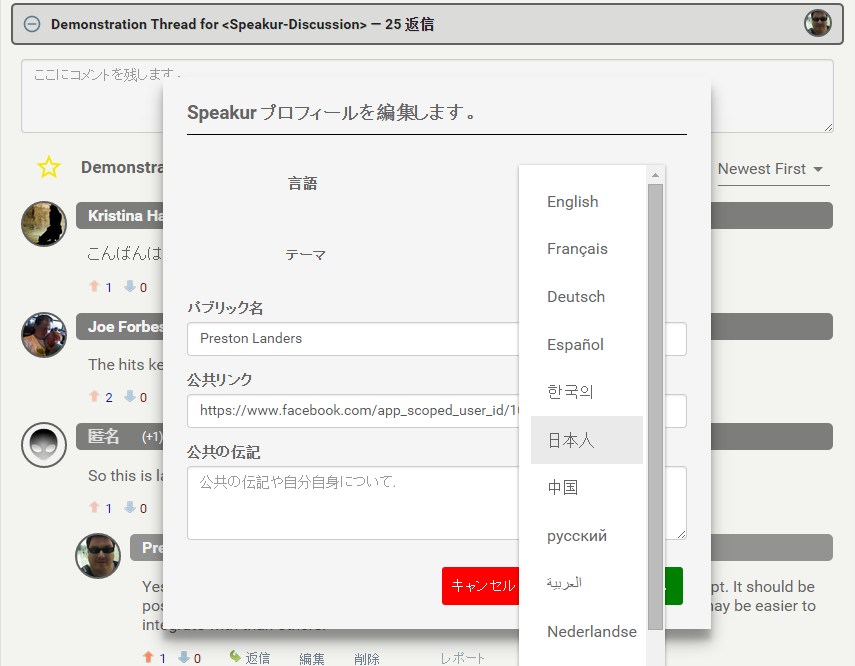
\includegraphics[width=5.5in]{images/screenshot_20150320_1923_lang.png}
\caption{Speakur's interface language\index{internationalization} updates instantly upon selection.}
\label{f:lang}
\end{figure}

From a technical perspective, one of the more interesting features in Speaker\index{Speakur} is the use of Polymer's\index{Polymer} data-bound templates\index{data-bound template}, also known as Model-Driven Views\index{Model-Driven View}, 
to allow components to automatically reflect changes in far-flung areas of the application.
Also, Firebase's\index{Firebase} event notification\index{event notification} architecture allows all web clients to instantly and transparently reflect any changes in another remote client.
Another example of the power of data-bound templates is that all of the user-visible text in the application updates immediately as soon as the user changes his or her locale preference in the dialog in Figure~\ref{f:lang}.

\section{Architecture Overview}
It has been said that ``any problem in computer science can be solved with another layer of indirection\index{indirection}'' (usually attributed to Wheeler).
The key to understanding a software package is learning its architecture\index{architecture},
which is really a map of these layers of indirection\index{indirection} and abstraction\index{abstraction}.
Roy Fielding, the author of the influential REST\index{REST} web architecture\index{architecture}, described a software architecture as:

\begin{quote}
\dots an abstraction of the run-time elements of a software system during some phase of its operation. A system may be composed of many levels of abstraction and many phases of operation, each with its own software architecture.

At the heart of software architecture is the principle of abstraction: hiding some of the details of a system through encapsulation\index{encapsulation} in order to better identify and sustain its properties. A complex system will contain many levels of abstraction, each with its own architecture~\cite{fielding2000}.
\end{quote}

The architecture for Speakur\index{Speakur} is based on client-side (browser) JavaScript\index{JavaScript} code and HTML\index{HTML} layout following Web Components\index{Web Components} design principles. 
There is no dedicated server component except for the Firebase\index{Firebase} cloud database service~\cite{firebasecontributors2015}.
Speakur is built entirely from plain HTML, JS and CSS\index{CSS} files that can be served from a content distribution network (CDN)\index{content distribution network (CDN)} 
such as \tcode{github.io}\index{GitHub} or your own server~\cite{landers2015-d}.

This low-overhead design allows Speakur\index{Speakur} to be used on your own website without actually `installing' any software;
just load Speakur directly from \tcode{github.io} with an HTML \textit{import}
and then insert a tiny bit of HTML markup into your document~\cite{landers2015-d}.
This helps fulfill the ease of use requirements 
\#\ref{motive:abstraction} and \#\ref{motive:cors}
in section~\ref{motivations}.

Most of the user interface\index{user interface (UI)} elements in Speakur\index{Speakur} 
--- things like dropdown menus and dialogs as well as invisible functional components like expand/collapse elements  
--- are implemented with Polymer's\index{Polymer} Core\index{Core Elements} and Paper\index{Paper Elements} custom element libraries.
Speakur presents a simple API through \tcode{<speakur-discussion>}\index{<speakur-discussion>},
but internally it consists of a number of internal abstraction layers or custom elements.
In turn, these internal layers consist of still more focused layers, other Polymer components, simple HTML templates, and wrappers around external JavaScript\index{JavaScript} libraries like  \tcode{moment.js}\index{moment.js library}.

As previously mentioned, in order to make the 
\tcode{<speakur-discussion>}\index{<speakur-discussion>} element available for use, you must first load the Web Components polyfill\index{polyfill} and then \textit{import} the Speakur element, either from \tcode{github.io} or your own server.
It is recommended to create your own Firebase\index{Firebase} instance for data security and resource limitation reasons, but even this is not required. 
The author's demonstration database will be used by default.

Security\index{security} for web clients engaging in data manipulation (i.e, posting, editing or deleting comments) is handled entirely through Firebase\index{Firebase} authentication\index{authentication} and data security\index{security} rules described below.
The simplicity of this arrangement means that it is extremely easy to fit Speakur into almost any web application architecture.

\section{Responsive Design}
Because Speakur\index{Speakur} is not a standalone application but rather a plug-in designed to be embedded into other web pages or apps, 
the full document is not under its control.
This can affect the mobile\index{mobile} user experience\index{user experience (UX)},
but within these limits, Speakur strives to present a responsive\index{responsive design} interface to different screen sizes.

The primary way it does this is...

\section{Polymer and Web Components}
As described in Chapter~\ref{ch:background}, 
Web Components\index{Web Components} are a 
W3C\index{W3C} initiative 
to expose certain native browser features in a public, standardized way. 
Polymer\index{Polymer} is a 
Google\index{Google} 
web framework built from the ground up around Web Components.
Polymer also provides the crucial Web Component 
polyfill\index{polyfill} library 
that is required for these features to work on most current browsers.

In general, Speakur tries to adhere to the core principles laid out by the 
Web Components\index{Web Components} developers 
for general purpose components. 
It's worth quoting those here in full, 
because they are applicable to software engineering\index{software engineering} in general. They are:

\begin{quote}
\begin{enumerate}
\item Address a common need.\label{wcp:commonneed}
\item Do one job really well.\label{wcp:onejob}
\item Work predictably in a wide variety of circumstances.\label{wcp:predicatable}
\item Be useful right out of the box.\label{wcp:useful}
\item Be composable.\label{wcp:composable}
\item Be styleable.\label{wcp:stylable}
\item Be extensible.\label{wcp:extensible}
\item Think small.\label{wcp:thinksmall}
\item Adapt to the user and device.\label{wcp:adaptable}
\item Deliver the key benefit to HTML authors, not just coders.\label{wcp:htmlauthors}
~\cite{webcomponentscontributors2014}
\end{enumerate}
\end{quote}

Explain how I follow those guidelines... [TODO]

The Polymer project provides two (optional) libraries of Custom Elements\index{Custom Elements} for use in your own projects. 
\textbf{Core Elements}\index{Core Elements} includes both user interface\index{user interface (UI)}
widgets and invisible functional elements.
Core Elements are minimally styled and can be used standalone, 
but they are also used as `base classes' for 
\textbf{Paper Elements}\index{Paper Elements}, 
which implement the so-called `Material Design'\index{Material Design} look and feel (design language) used by apps for Google's\index{Google} Android\index{Android} mobile\index{mobile} operating system~\cite{imura2015}.
Speakur's\index{Speakur} layout is composed of native HTML5 elements, 
Core and Paper Elements, 
and Speaker's own custom elements that are used to abstract\index{abstraction} internal implementation details.

\section{Data store and synchronization}
All persistent data in Speakur is stored in a cloud database called Firebase~\cite{firebasecontributors2015}\index{Firebase}.
Anyone who wants to use Speakur\index{Speakur} can register for a free account on \tcode{firebase.com} and create a database instance to hold Speakur data.
No other server component is required.
Firebase is a NoSQL\index{NoSQL}-style key-value data store of the kind that has been popularized
with the growth of 
Node.js\index{Node.js}, a server-side JavaScript\index{JavaScript} environment,
and the MongoDB\index{MongoDB} NoSQL database~\cite{dickey2014}.

Firebase\index{Firebase} provides WebSockets\index{WebSockets}-based event notification and synchronization 
as well as a security rule description format based on 
JSON\index{JSON}\footnote{JavaScript Object Notation (JSON)\index{JSON} is a popular alternative to XML because it is more easily human-readable. 
It mirrors the syntax for writing data structure literals in the JavaScript\index{JavaScript} language.} 
for securing\index{security} and validating user actions.
The use of Firebase as the only server component allows for easy deployment of Speakur with minimal dependencies, helping to keep the component small and focused.

\subsection{Firebase API}
Firebase\index{Firebase} can be used `standalone' as the sole provider of data services to an application, as Speakur does, or else it can be used as an auxiliary to other services or REST\index{REST} APIs\index{API}.
One of the key architectural benefits of using Firebase, 
besides its ease of deployment, 
is that its data binding and event notification system allows for 
applications to respond to changes in real-time while remaining performant.

Firebase itself provides a REST API for data access by programs like Speakur.
The term REST or RESTful is sometimes misunderstood,
but in Roy Fielding's original 2000 Ph.D. thesis, 
REST refers to transferring \textit{representations} of application state and using hypertext as the engine of 
application state\index{HATEOAS}\footnote{Known under the somewhat awkward acronym of HATEOAS\index{HATEOAS}.}.
Specifically, `objects' of whatever type are represented as interlinked hypertext \textbf{\textit{resources}} that are operated on by standard HTTP verbs\index{HTTP!verbs} such as PUT\index{HTTP!PUT} and DELETE\index{HTTP!DELETE}.

Areas where typical web APIs\index{API} fall short of being truly ``REST-ful''\index{REST} include:
\begin{enumerate}
\item Treating URLs as endpoints for remote procedure calls (RPC\index{RPC}) instead of hypertext resources that are interlinked in exactly the same way a website is like a tree that starts from the home page and links to various resources.
\item Using HTTP verbs\index{HTTP!verbs} inappropriately, such as using POST for all actions including deletion.
\item Not using content related HTTP headers\index{HTTP!headers} appropriately for data representation and API versioning\index{versioning}~\cite{steveklabnik2011}.
\end{enumerate}

The Firebase API follows typical RESTful\index{REST} patterns in data access, allowing the database and its metadata to be addressed as a set of linked HTTP resources.
In addition, Firebase client libraries use WebSockets\index{WebSockets}, 
a lower-level TCP/IP protocol, 
to perform event notification and distributed synchronization without the overhead of polling or high-overhead HTTP 1.1\index{HTTP} requests.
WebSockets\index{WebSockets} are used for performance reasons but all of the data in Firebase\index{Firebase} (and hence, in Speakur\index{Speakur}) is accessible from the RESTful\index{REST} HTTP API\index{API} outside of a WebSocket\index{WebSockets}.

\subsection{WebSockets}
\label{sec:websockets}
The WebSockets\index{WebSockets} protocol, formally known as RFC 6455\index{RFC 6455}, is a TCP/IP\index{TCP/IP} protocol that can be used alongside HTTP\index{HTTP} for persistent data connections between web clients and servers~\cite{mozillacontributors2015-a}.
The primary purpose is to avoid the overhead of initiating a new HTTP connection to check on the status of something on the server, also known as polling\index{polling}.
Firebase\index{Firebase} uses Web Sockets rather than traditional high-overhead HTTP\index{HTTP} requests to move data back and forth to the client.
This always-on connection allows for sending nearly instant event notifications to all currently active clients with minimal overhead.
In practice, this allows the application to update its state in real-time as different users read and write values the database.
The Firebase client library 'subscribes' to an area of interest in the database, such as the replies to a particular thread, and receives notifications when these areas change and updates the local representation as appropriate.

\section{Security}
Because Speakur\index{Speakur} relies entirely on Firebase\index{Firebase} for data persistence, that means its security model is largely built around Firebase. 
All Speakur code runs inside the client's web browser including the small `admin' mode.
The security architecture\index{architecture} of the web is largely based around protecting the \textit{user} from malicious servers and other users, not protecting the \textit{server} from the user.
The server has to take its own steps to protect itself from unauthorized actions.
Speaker has no 'server' as such other than the Firebase cloud service.
That means the security mechanisms that do things like prevent users from deleting each other's posts are implemented entirely within Firebase security rules as discussed in section~\ref{sec:security}.
Confidentiality of data in-transit is handled with the same Transport Layer Security (TLS)\index{transport layer security (TLS)} better known as the secure socket layer (SSL)\index{secure socket layer (SSL)} or HTTPS\index{HTTP!HTTPS}.

Firebase implements the two major categories of access control: authentication\index{authentication} and 
authorization\index{authorization}. 
Authentication (sometimes abbreviated \textit{authn}) answers the question ``who are you?'' 
while authorization (\textit{authz}) asks ``what are you allowed to see and do?''~\cite{stallings2011}.


\subsection{Authentication}

Speakur's authentication\index{authentication} and sign-in system is handled through Firebase\index{Firebase}, 
specifically Google\index{Google} and Facebook\index{Facebook} OAuth\index{OAuth} single-sign on (SSO)\index{single sign-on (SSO)}.
Users can sign into a Speakur discussion thread, and hence Firebase, through their Facebook or Google identity.
Firebase\index{Firebase} supports other authorization schemes, including account registration (``simple password''), Twitter\index{Twitter} and GitHub\index{GitHub} identities.
Site owners who use Speakur can also designate certain threads to allow anonymous commenting.

Every user who registers within a Speakur\index{Speakur} instance by signing in with one of those identity providers gets a unique identifier --- the \tcode{uid} or user ID. 
This \tcode{uid} is used extensively in the database to refer to the user, including in the security (authorization\index{authorization}) rules that are external to the actual database (i.e, security metadata\index{metadata}.) 

\subsection{Authorization}
Authorization\index{authorization} rules determine what level of access a user has within the system, or what they are allowed to do or see.


\section{Data Flow and Event Handling}

\subsection{Mutation Observers}

\section{Dependencies and Deployment}

Bower\index{Bower}

Vulcanize\index{Vulcanize}

CORS\index{Cross-origin resource sharing (CORS)}

